\pdfoutput=1

\documentclass[3p,times]{elsarticle}

\makeatletter
\def\ps@pprintTitle{%
 \let\@oddhead\@empty
 \let\@evenhead\@empty
 \def\@oddfoot{}%
 \let\@evenfoot\@oddfoot}
\makeatother

\journal{}

% *** GRAPHICS RELATED PACKAGES ***
\usepackage{graphicx}
\usepackage{pgfplots}
\usepackage{float}
\usepackage{caption}
\usepackage{subcaption}

% *** MATH PACKAGES ***
\usepackage{amsmath}
\usepackage{amssymb}
\usepackage{bm}
\usepackage{amsthm}

% *** SPECIALIZED LIST PACKAGES ***
\usepackage{algorithm,algpseudocode}
\renewcommand\algorithmicdo{until convergence}
\renewcommand\algorithmicfor{For}
\algtext*{EndFor}

% *** ALIGNMENT PACKAGES ***
\usepackage{array}

% *** PDF, URL AND HYPERLINK PACKAGES ***
\usepackage{url}

% *** TABLES PACKAGES ***
\usepackage{booktabs}

% *** BIBLIOGRAPHY PACKAGES ***
\usepackage[numbers]{natbib}

\begin{document}

\begin{frontmatter}

\title{Parameters Optimisation of Support Vector Data Description with Radial Basis Function Kernel for Anomaly Detection in Wireless Sensor Networks}

\author[donga]{Van Vuong~Trinh\corref{cor1}}
\cortext[cor1]{Corresponding author}
\ead{vanvuong.trinh@gmail.com}

\author[donga]{Kim Phuc~Tran}
\ead{kimphuc.tran@gipsa-lab.fr}

\author[hust]{Anh Tuan~Mai}
\ead{mtuan@itims.edu.vn}

\address[donga]{Dong A University, Vietnam}  
\address[hust]{International Training Institute for Materials Science (ITIMS)\\Hanoi University of Technology, Vietnam} 

\begin{keyword}
anomaly detection, support vector data description, derivative-free optimization, wireless sensor networks.
\end{keyword}

\begin{abstract}
\end{abstract}

\end{frontmatter}

\section{Introduction}

\section{Support Vector Data Description with Radial Basis Function Kernel}

In this section, let us briefly describe the support vector data sescription (SVDD) originally derived in \cite{Tax2004} which is an alternative of the known one-class support vector classifiers \cite{Scholkopf2000} and analogous to support vector machines (SVM) \cite{Vapnik1998}.

Given training data

In the following the target objects are enumerated by indices $i$, $j$ and the negative examples by $l$, $m$. For further convenience assume that target objects are labeled $y_i=1$ and outlier objects are labeled $y_l=−1$. Again we allow for errors in both the target and the outlier set and introduce slack variables $\xi_i$ and $\xi_l$.

Primal optimisation which is a quadratically constrained quadratic program (QCQP) (and is equivalent to second-order cone program (SOCP) by trivial changing decision variables):
\begin{subequations}\label{eq:svdd_primal}
\begin{align}
\underset{
	\begin{array}{c}
		 R, \mathbf{a}, \xi_i
	\end{array}}{\text{Minimize }} & F = R^2 + C \sum_i \xi_i \\
\text{Subject to } & \left|\left| \mathbf{x}_i - \mathbf{a} \right|\right|^2 \le R^2 + \xi_i, \quad \xi_i \ge 0 \quad \forall i
\end{align}
\end{subequations}

Dual optimisation is a standard quadratic program (QP) which can be solved efficiently.
\begin{subequations}\label{eq:svdd_dual}
\begin{align}
\underset{
	\begin{array}{c}
		 \alpha_i, \alpha_l
	\end{array}}{\text{Maximize }} & L = \sum_i \alpha_i \left( \mathbf{x}_i \cdot \mathbf{x}_i \right) - \sum_{i,j} \alpha_i \alpha_j \left( \mathbf{x}_i \cdot \mathbf{x}_j \right)\\
\text{Subject to } & 0 \le \alpha_i \le C \quad \forall i
\end{align}
\end{subequations}

To test an object $\mathbf{z}$, the distance to the center of the sphere has to be calculated. A test
object $\mathbf{z}$ is accepted when this distance is smaller or equal than the radius:
\begin{align}
\left|\left| \mathbf{z} - \mathbf{a} \right|\right|^2 = \left( \mathbf{z} \cdot \mathbf{z} \right) - 2 \sum_i \alpha_i \left( \mathbf{z} \cdot \mathbf{x}_i \right) + \sum_{i,j} \alpha_i \alpha_j \left( \mathbf{x}_i \cdot \mathbf{x}_j \right)
\end{align}

By definition, $R^2$ is the distance from the center of the non-spherical $\mathbf{a}$ to (any of the support vectors on) the boundary. Support vectors which fall outside the description are excluded. Therefore:
\begin{align}
R^2 = \left( \mathbf{x}_k \cdot \mathbf{x}_k \right) - 2 \sum_i \alpha_i \left( \mathbf{x}_i \cdot \mathbf{x}_k \right) + \sum_{i,j} \alpha_i \alpha_j \left( \mathbf{x}_i \cdot \mathbf{x}_j \right)
\end{align}
for any $\mathbf{x}_k \in SV_{<C}$, the set of support vectors which have $\alpha_k < C$.

\section{Parameters Optimisation Algorithm via Bilevel Programming}

\cite{scholkopf2001estimating}

\cite{theissler2013autonomously}

\begin{align}
\dfrac{1}{N} \le C \le \min \left( 1, \dfrac{1}{\nu N} \right)
\end{align}

$\nu$ fraction outlier

\begin{subequations}
\begin{align}
\underset{
	\begin{array}{c}
		 C, \sigma
	\end{array}}{\text{Minimize }} & J\left( C, \sigma \right)\\
\text{Subject to } & \dfrac{1}{N} \le C \le \min \left( 1, \dfrac{1}{\nu N} \right) \\
& 0 \le \sigma
\end{align}
\end{subequations}

\section{Application to Anomaly Detection in a Wireless Sensor Networks}

\subsection{Intel Berkeley Research Laboratory Data}

We consider a data set gathered from a wireless sensor network deployment at the Intel Berkeley Research Laboratory (IBRL) \cite{Buonadonna2005}. A wireless sensor network consisting of $54$ \emph{Mica2Dot} sensor nodes was deployed in the IBRL for a $30$ day ($720$ hour) period between 28th Feb 2004 and 5th April 2004 [10]. Figure~\ref{fig:ibrl_wsn} shows the deployed node locations in the laboratory. The sensors collect five measurements: light in Lux, temperature in degrees celsius, humidity (temperature corrected relative humidity) ranging from $0\%$ to $100\%$, voltage in volts and network topology information in each $30$ second interval. Node $0$ is the gateway node. Other nodes transmit their data in multiple hops to the gateway node. The furthest node in the network is about $10$ hops away from the gateway node. During the $30$ day period, the $54$ nodes collected about $2.3$ million readings.

\begin{figure}[H]
\centering
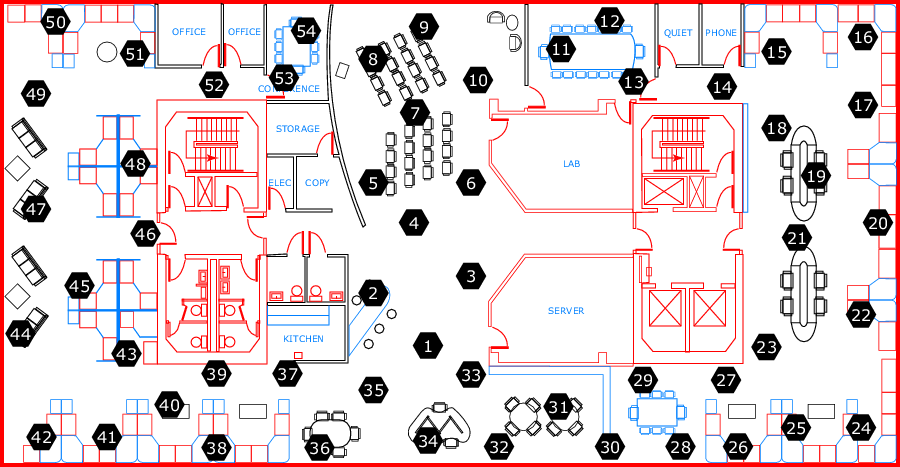
\includegraphics[scale=.3]{Pictures/ibrl_wsn}
\caption{A map of IBRL, with mote locations labeled in black.}
\label{fig:ibrl_wsn}
\end{figure}

In this paper we consider the IBRL data set obtained from $54$ nodes, namely node IDs from $1$ to $54$, during the first $10$ days period collected on March 2004. While the lab in Figure~\ref{fig:ibrl_wsn} has a total of $55$ sensors (including the gateway node), only $54$ of them provided data during the $10$ days time window examined in this paper. Also, only two features, namely temperature and humidity, are taken into account. However, since node $M_5$ did not contain any humidity data during this time window, we only 

It is notable that the notes contain a number of outliers.

Nodes $15$ and $18$ provided unrealistic data during some time intervals, i.e. too high or too low. 

\subsection{Numerical Analysis of Parameters Optimization Algorithm}

Platform: 2.6 GHz Intel(R) Core(TM) i7 and 16GB of RAM.
IBM ILOG CPLEX 12.7.0

\section{Conclusion and Future Work}

\bibliographystyle{IEEEtran}
\bibliography{wsnbib,svmbib,ocsvmbib,ibrlbib,miscbib}

\end{document}


